
\begin{frame}{\citetitle{MarcoNuno_Revista_2022_10_00}$^*$ (1)}
\begin{columns}
\begin{column}{0.99\textwidth}
	\begin{itemize}  %del cuerpo académico Acuicultura Sustentable (UTMTB-CA-1)
        \item Una aplicación eficaz para uso de transporte publico debe mostrar información acerca de las opciones de movilidad el usuario tiene en una localidad específica.
        \item En algunas localidades, esta información no esta disponible en las aplicaciones de mapas, lo que complica la movilidad del usuario.
		\item Se implementó una App específicamente para Ciudad Victoria, Tamps
	\end{itemize}
\end{column}
%\begin{column}{0.25\textwidth}  
%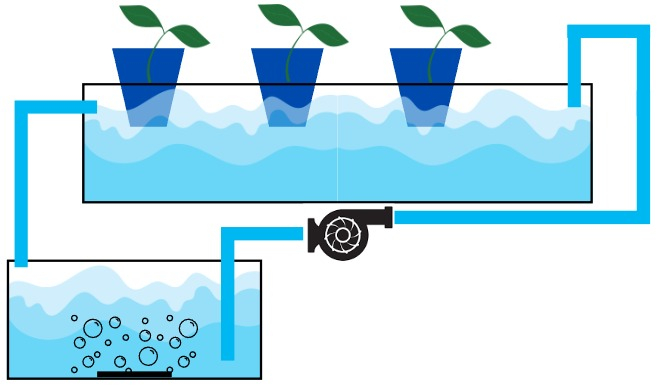
\includegraphics[width=0.98\textwidth]{2022_HidroponicosDavid/figs/dft}
%\end{column}
%\begin{column}{0.25\textwidth}
%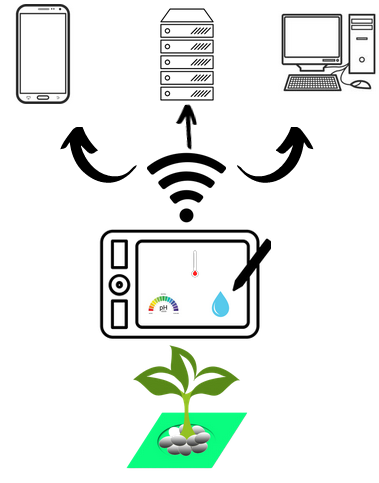
\includegraphics[width=0.98\textwidth]{2022_HidroponicosDavid/figs/iot}
%\end{column}
\end{columns} 
\footfullcite*{MarcoNuno_Revista_2022_10_00}
\end{frame}


\begin{frame}{\citetitle{MarcoNuno_Revista_2022_10_00} (2)}
\begin{columns}
\begin{column}{0.25\textwidth}  
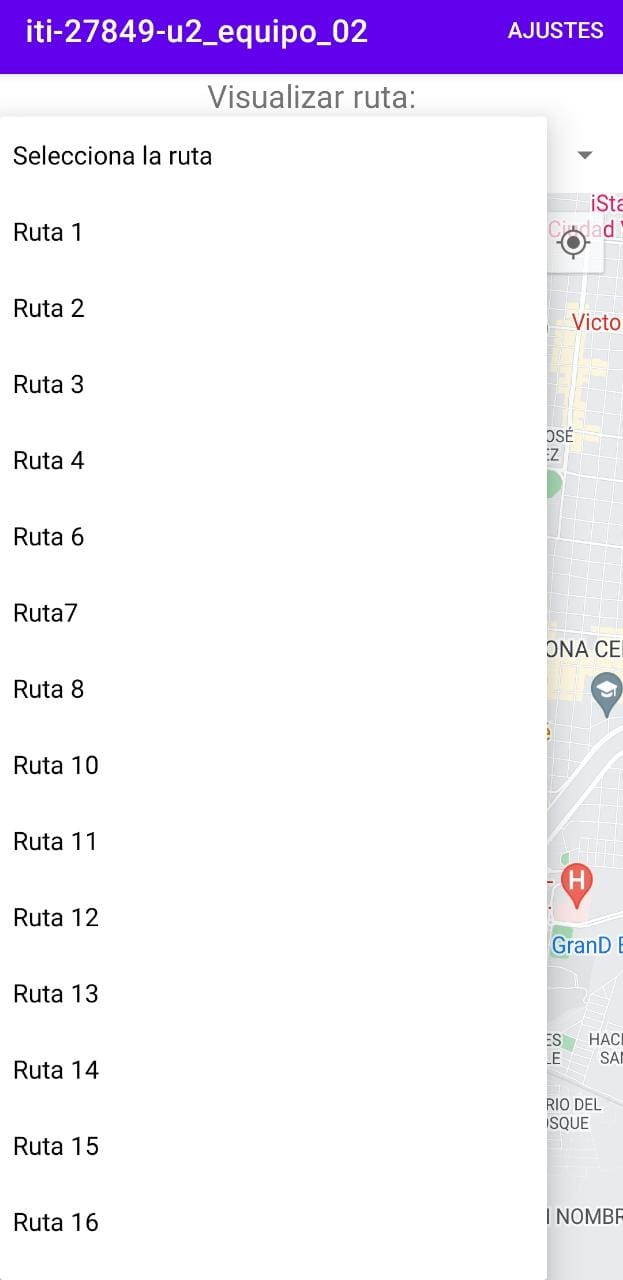
\includegraphics[width=0.82\textwidth]{2022_MapaVickyRanch/figs/F3}
\end{column}
\begin{column}{0.25\textwidth}  
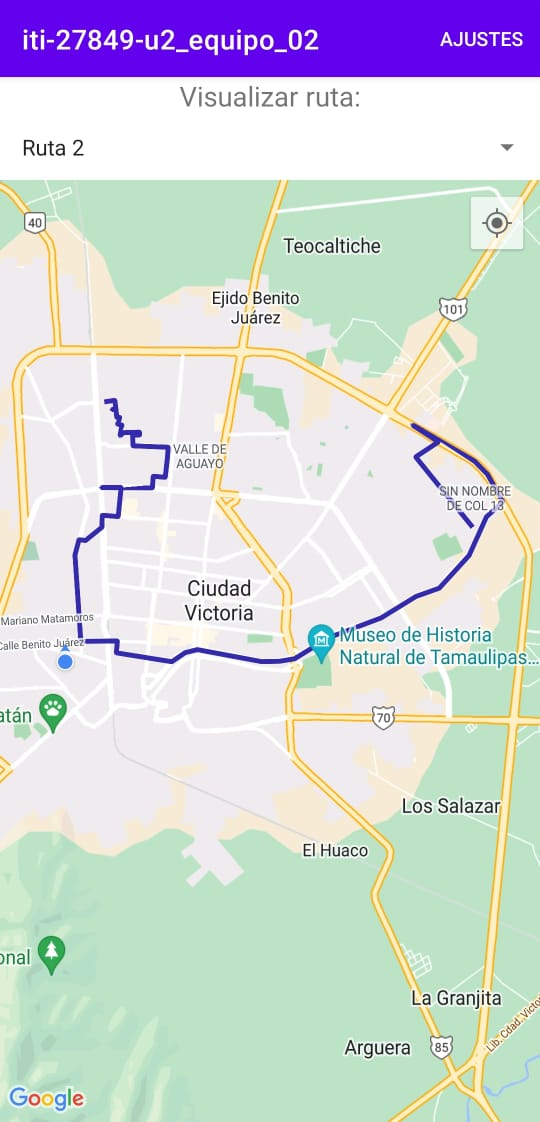
\includegraphics[width=0.82\textwidth]{2022_MapaVickyRanch/figs/F4}
\end{column}
\begin{column}{0.25\textwidth}  
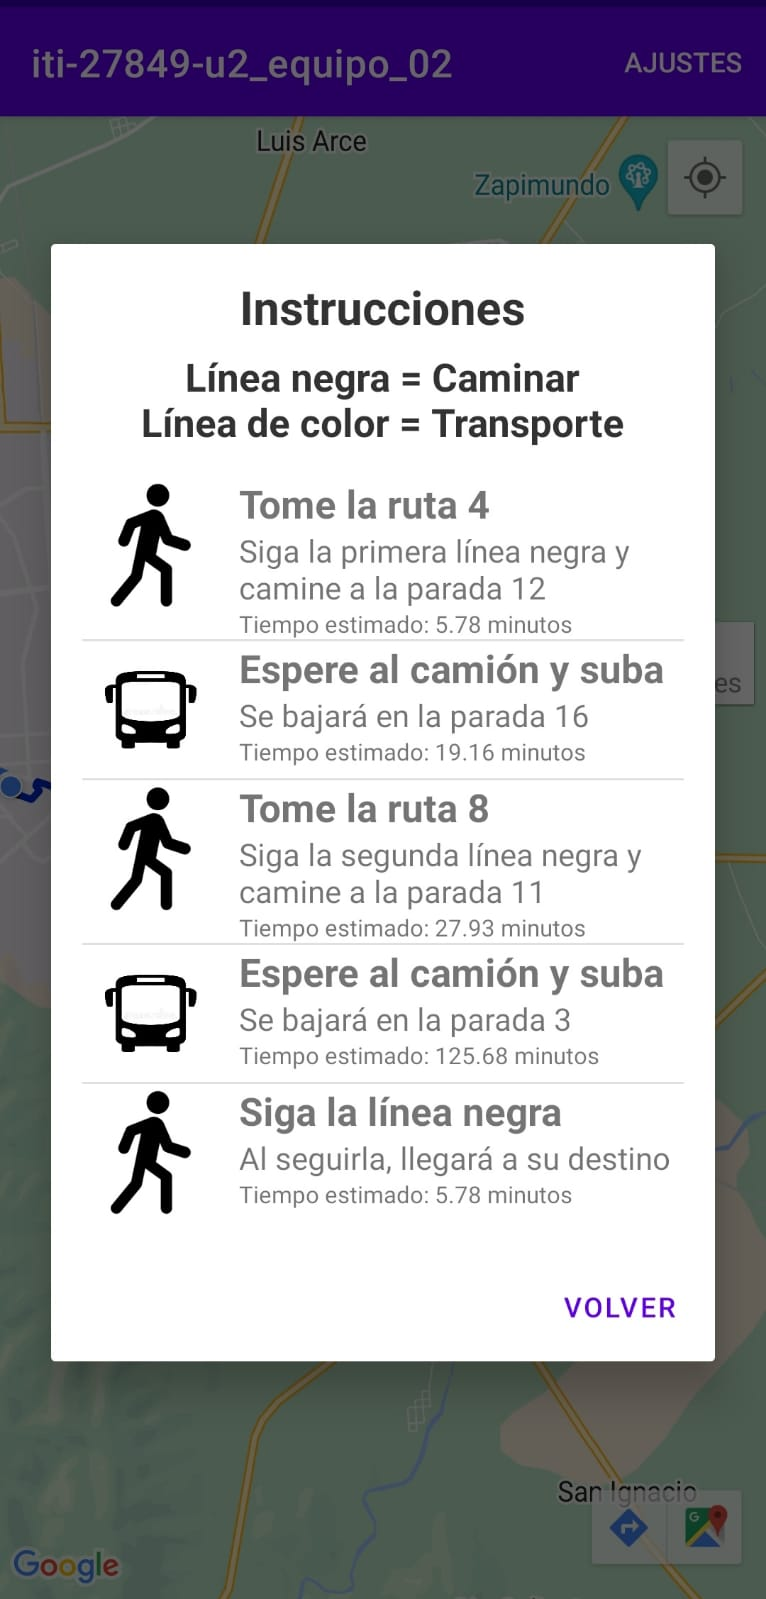
\includegraphics[width=0.82\textwidth]{2022_MapaVickyRanch/figs/F9}
\end{column}
\begin{column}{0.25\textwidth}  
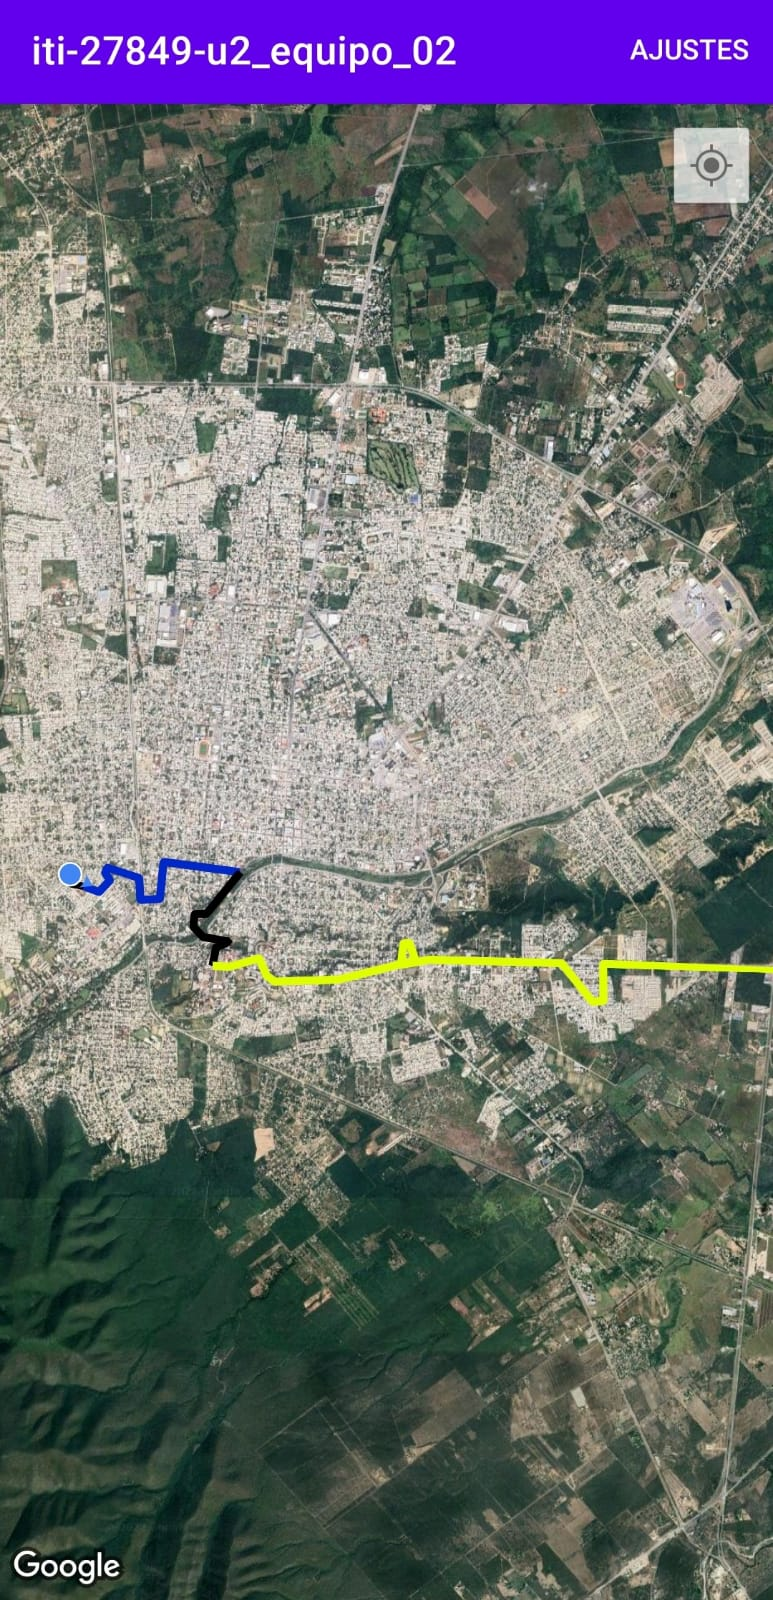
\includegraphics[width=0.82\textwidth]{2022_MapaVickyRanch/figs/F13}
\end{column}

\end{columns} 
\end{frame}

